\documentclass[10pt,twoside]{article}

% ---------------------------------------------------------------- page
\usepackage[a4paper,left=1.05in,right=1.05in,top=1.15in,bottom=1.15in]{geometry}
\usepackage[T1]{fontenc}
\usepackage[utf8]{inputenc}

% Palatino text with matching math -- a deliberate choice rather than the
% Computer Modern default: it sets denser and reads better at 10pt.
\usepackage{mathpazo}
\linespread{1.06}

\usepackage{amsmath,amssymb}
\usepackage{graphicx}
\usepackage{booktabs}
\usepackage{natbib}
\usepackage{xcolor}
\usepackage{microtype}

% ---------------------------------------------------------------- headings
\usepackage{titlesec}
\titleformat{\section}{\normalfont\large\bfseries}{\thesection}{0.7em}{}
\titleformat{\subsection}{\normalfont\normalsize\bfseries}{\thesubsection}{0.7em}{}
\titlespacing*{\section}{0pt}{2.0ex plus .4ex minus .2ex}{1.0ex plus .2ex}
\titlespacing*{\subsection}{0pt}{1.6ex plus .3ex minus .2ex}{0.7ex plus .2ex}

% ---------------------------------------------------------------- floats
\usepackage{caption}
\captionsetup{font=small,labelfont=bf,labelsep=period,justification=justified}

% ---------------------------------------------------------------- running head
\usepackage{fancyhdr}
\pagestyle{fancy}
\fancyhf{}
\fancyfoot[C]{\small\thepage}
\renewcommand{\headrulewidth}{0pt}
\fancypagestyle{plain}{\fancyhf{}\fancyfoot[C]{\small\thepage}%
  \renewcommand{\headrulewidth}{0pt}}

% ---------------------------------------------------------------- line numbers
% Reviewers ask for these; comment out for a clean reading copy.
\usepackage{lineno}
\linenumbers
\renewcommand\linenumberfont{\normalfont\tiny\color{gray}}

\usepackage[colorlinks=true,allcolors=black,citecolor=black,
            urlcolor=blue!45!black]{hyperref}

\newcommand{\cell}[1]{\texttt{#1}}

% ---------------------------------------------------------------- title block
\makeatletter
\renewcommand{\maketitle}{%
  \thispagestyle{plain}
  \begin{center}
    {\LARGE\bfseries \@title \par}\vspace{1.1em}
    {\large \@author \par}\vspace{0.5em}
    {\small \@date \par}
  \end{center}
  \vspace{0.6em}
}
\makeatother

\title{FlyDoom: A frozen whole-brain \emph{Drosophila} connectome\\[3pt]
in a closed sensorimotor loop}

\author{Mehmet Utku \"Ozt\"urk\\[3pt]
{\normalsize Independent researcher}\\
{\small\texttt{mutkuoz@proton.me}}}
\date{\today}

\begin{document}
\maketitle

\begin{abstract}
\noindent
Synapse-resolution connectomics permits simulation of an entire brain with
essentially no free parameters, but such models are typically driven open loop.
We embed a frozen FlyWire FAFB v783 connectome (139{,}255 neurons; 2{,}710{,}038
edges) in a closed sensorimotor loop with a video game. No parameter is trained,
and the only fitted quantity is a single global synaptic gain calibrated on a
non-visual behaviour.

Transfer is dissociated by modality. Chemosensory transformations are
reproduced: sugar stimulation drives the proboscis motor pool to 77\,Hz,
co-stimulation with bitter is 99\% suppressed, and an olfactory channel raises
lateral horn activity to $14.1\pm5.5$\,Hz while suppressing a descending neuron
one synapse downstream ($-17.7\pm7.4$\,Hz), none of which was fitted and none of
which survives a degree-preserving shuffle. Visual motion computation is not
reproduced: $|\mathrm{DSI}|\leq0.0121$ across an operating-point sweep, roughly
$40\times$ below the threshold at which experimental studies classify a terminal
as direction-tuned.

We identify the obstacle as a property of the neuron model rather than of the
connectome. Direction selectivity requires a multiplicative interaction between
the correlator arms, which in a conductance-based neuron must arise from
inhibitory division. That division cancels itself: shunting divides the membrane
by $g_{\mathrm{tot}}$ ($1.77\times$ at \cell{T4a}) while the accompanying
hyperpolarisation raises the excitatory driving force by $1.85\times$, leaving
an interaction below 11\% and of the wrong sign. The cell sums its inputs, and
summation cannot be direction selective at any wiring.

Increasing the inhibitory-to-excitatory conductance ratio restores the
interaction. Applied globally it inverts the gustatory result, driving the
proboscis pool to 168\,Hz under bitter stimulation, because 51\% of inhibitory
synapses terminate on inhibitory neurons. Applied to the visual populations
alone, the same factor leaves the gustatory circuit numerically unchanged,
preserves olfaction, increases direction selectivity sevenfold, and yields
behaviour: on thirty held-out environment seeds the model exceeds a
command-matched control on ten of eighteen measures, where the frozen model
exceeds it on none.

A single global synaptic gain is therefore not merely incomplete but
inconsistent: the optic lobe requires a conductance ratio the subesophageal zone
does not tolerate. Published physiology places the optic lobe requirement in the
same range. We additionally report that degree-preserving shuffle controls are
invalid in closed loop, because the two arms sample different stimulus
distributions.
\end{abstract}

\vspace{0.4em}
\noindent\textbf{Keywords:} connectomics; \emph{Drosophila}; whole-brain
simulation; closed-loop embodiment; elementary motion detection; olfactory
valence; negative results

\vspace{0.8em}
\hrule
\vspace{1.2em}

\section{Introduction}

An electron-microscopy reconstruction of an adult \emph{Drosophila} brain now
provides every chemical synapse between all 139{,}255
neurons~\citep{dorkenwald2024}, together with cell-type annotation
\citep{schlegel2024} and per-synapse neurotransmitter
prediction~\citep{eckstein2024}. This raises a question that was previously
unaskable: \emph{how much of an animal's behaviour is implied by its wiring
alone?}

Two recent lines of work answer parts of it, and they answer differently.
\citet{shiu2024} built a whole-brain leaky integrate-and-fire model with a
uniform parameter set and a single fitted scalar, the per-synapse weight
$W_{\mathrm{syn}}$, and recovered gustatory behaviours such as
proboscis extension. \citet{lappalainen2024} built a connectome-\emph{constrained}
model of 64 optic-lobe cell types in which the unknown biophysical parameters
were \emph{optimized} by gradient descent on a motion-estimation task, and
recovered single-neuron responses matching 26 experimental studies. These
differ in two ways at once: whole-brain versus optic lobe, and frozen versus
optimized.

Both are driven open loop. \citet{wangchen2024} close the loop, embedding the
optimized visual network of \citet{lappalainen2024} in a biomechanical fly with
reinforcement-learned controllers. The configuration that has not been tested
is the remaining corner: a \emph{whole-brain, frozen, unoptimized} connectome
placed in a closed sensorimotor loop.

That corner is informative precisely because of the contrast. If a frozen
whole-brain model reproduces a computation, the wiring plus a global gain
sufficed. If it fails at a computation that the optimized model achieves on the
same wiring, the difference isolates what optimization supplied.

We report such a test. We drive the frozen connectome with the rendered frames
of \emph{Doom}~\citep{kempka2016}, read eight characterized
descending neurons, and return their activity to the game as control input, in
real time. The environment is adversarial and non-stationary but, crucially
for interpretation, entirely outside the fly's evolutionary experience, so
nothing here is a test of ecological competence. It is a test of which
sensorimotor transformations survive the transfer from wiring diagram to
running system.

\paragraph{Contributions.}
\begin{enumerate}\itemsep2pt
\item A closed-loop embodiment of a frozen whole-brain connectome
(139{,}255 neurons, single consumer GPU or CPU), released as open code, running
at $0.19\times$ realtime.
\item A modality dissociation: chemosensory transformations transfer, visual
motion computations do not.
\item A mechanistic account of the visual failure. Twenty candidate
explanations were implemented and measured; the operative one is that shunting
inhibition cancels itself, so the neuron sums its inputs where the computation
requires a product.
\item A demonstration that a single global synaptic gain is inconsistent rather
than merely approximate. Raising the inhibitory-to-excitatory ratio restores
the multiplicative interaction, but the optic lobe requires a value the
subesophageal zone does not tolerate; applied regionally the same factor
increases direction selectivity sevenfold at no cost to the chemosensory
results, and produces closed-loop behaviour that separates from a
command-matched control on ten of eighteen measures over held-out environment
seeds.
\item A positive result that beats a degree-preserving shuffle: an olfactory
channel reaches descending neurons through the anatomically named route with the
wiring-predicted sign.
\item A methodological caution: shuffle controls are invalid in closed loop.
\end{enumerate}

\section{Results}

\subsection{Model and closed-loop configuration}
\label{sec:model}

\begin{figure}[t]\centering
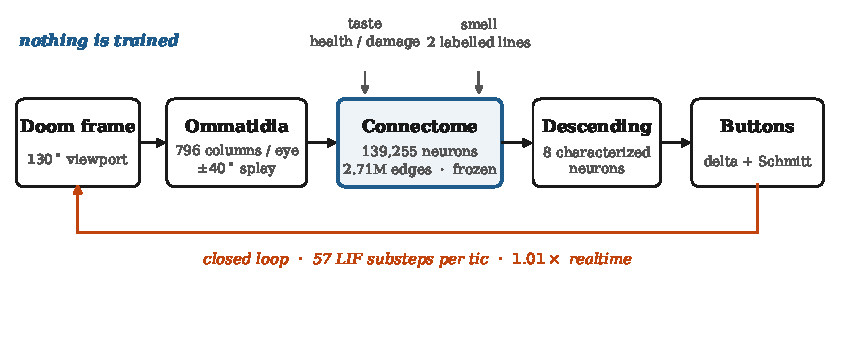
\includegraphics[width=\textwidth]{figs/fig1_pipeline.pdf}
\caption{The closed loop. Rendered frames are sampled by the real ommatidial
lattice, propagated through the frozen connectome for 57 leaky
integrate-and-fire substeps per game tic, and read out at eight characterized
descending neurons whose activity becomes the next action. Taste and smell
enter as direct drive on gustatory and olfactory receptor neurons. No component
is trained and no parameter is fitted to the environment.}
\label{fig:pipeline}
\end{figure}

We load FlyWire FAFB v783 and retain edges of at least five synapses, giving
2{,}710{,}038 edges carrying 31{,}578{,}726 synapses among 134{,}013 connected
neurons (Table~\ref{tab:graph}). Signs follow the predicted transmitter, with
glutamate treated as \emph{inhibitory}: it acts through GluCl chloride
channels in flies~\citep{cleland1996} and accounts for 16.6\% of the edges we
simulate (19.5\% before thresholding), so importing the vertebrate convention
would mis-sign about a sixth of the brain.

We sign per edge rather than per neuron, and in this pipeline the choice is not
free. Transmitter is predicted per synapse and reported per neuropil, so one
neuron can carry different predictions in different neuropils: 42{,}078 of the
128{,}972 presynaptic neurons in the simulated graph (32.6\%) carry more than
one, and 26{,}781 (20.8\%) carry both signs. Collapsing each neuron to a
synapse-weighted majority, the usual way of imposing Dale's law, would
flip 3.1\% of edges and 2.6\% of synapses. This matters for reading the
literature as much as for the model: the alternative Princeton release has
Dale's law applied upstream (0 of its 139{,}003 presynaptic neurons carry more
than one transmitter), so per-neuron and per-edge signing coincide there and
not here, and transmitter statistics quoted from one release do not describe
the other.

Photoreceptors required an explicit override. They release
histamine~\citep{hardie1989}, which is not among the six transmitters the
classifier predicts; on \cell{R1-6} output edges the classifier returns ACh
71.2\%, Glu 20.2\%, GABA 5.8\%, and every excitatory call yields the wrong sign
for a histaminergic chloride synapse. We force all photoreceptor output
inhibitory, flipping 11{,}920 of 18{,}437 edges. Without this the optic lobe processes a
contrast-inverted image.

\begin{table}[t]\centering\small
\caption{Graph as simulated. Unthresholded synapse count matches the figure
published for this release, confirming the extraction.}
\label{tab:graph}
\begin{tabular}{lr}
\toprule
Neurons (annotated) & 139{,}255\\
Edges, unthresholded & 16{,}847{,}997\\
Synapses, unthresholded & 54{,}492{,}922\\
\midrule
Edges simulated ($\geq5$ synapses) & 2{,}710{,}038\\
Synapses simulated & 31{,}578{,}726\\
Neurons with $\geq1$ edge & 134{,}013\\
Graded (non-spiking) units & 77{,}873\\
\midrule
Resident GPU memory & 31\,MB\\
GPU kernel time per 0.5\,ms step & ${\sim}310\,\mu$s\\
Wall-clock per 0.5\,ms step & $1.4$\,ms (CPU, 8 threads, CSR delivery)\\
Closed-loop rate & $0.19\times$ realtime\\
\bottomrule
\end{tabular}
\end{table}

Neurons are leaky integrate-and-fire with the parameters of \citet{shiu2024},
themselves drawn from \citet{kakaria2017}: $V_{\mathrm{rest}}=-52$\,mV,
$V_{\mathrm{thresh}}=-45$\,mV, $\tau_{\mathrm{mem}}=20$\,ms,
$\tau_{\mathrm{syn}}=5$\,ms, $t_{\mathrm{refrac}}=2.2$\,ms,
$t_{\mathrm{delay}}=1.8$\,ms. We integrate the linear subthreshold system
exactly rather than by forward Euler, which we measured 6\% low on a single
postsynaptic potential. At $dt=0.5$\,ms this gives 57 substeps per game tic,
with the frame held across all 57.

Vision enters through the real retinotopy: \texttt{column\_assignment} supplies
796 ommatidial columns per eye on a hexagonal lattice. Each column samples the
rendered frame through a Gaussian acceptance function, implemented as a
separable pre-blur followed by bilinear sampling at that column's gaze
direction. The engine draws a planar perspective projection, so a column at
azimuth $\theta$ is sampled at screen coordinate $\tan\theta/\tan(\mathrm{FOV}/2)$
rather than linearly in $\theta$; the linear map misplaces a column at
$10^\circ$ of gaze by 87\% and one at $30^\circ$ by 71\%, converging only at
the very edge of the viewport. Since retinotopy is the substrate every motion
computation runs on, and a warp of that size makes the angular spacing between
neighbouring columns vary about twofold across the field, we note it as a
correctness requirement rather than a refinement: rigid motion of the world
then sweeps the retina at a speed that depends on where one looks, which is
precisely the input a correlator tuned to a fixed spacing cannot use. The two
eyes are splayed $\pm40^\circ$; collapsing them onto the
screen centre makes both eyes see the same image and drives the left--right
steering difference to zero by construction. The engine's field of view must
be set through the
console rather than the command line, passing \texttt{+fov} is silently
ignored, and renders at $90^\circ$, $130^\circ$ and $160^\circ$ are
bit-identical, and it resets with each episode. At $130^\circ$ the viewport
covers 64\% of the lattice and at $160^\circ$, 80\%; remaining columns are
filled with the frame's mean luminance, because a dark surround is a permanent
high-contrast edge that the looming detectors report as a stationary object.

Frames are not held across the substeps of a tic. Doom draws at 35\,Hz and the
simulator runs 57 substeps per frame, so a held frame presents the retina with
a step change followed by 56 substeps of exactly zero temporal derivative,
while the delayed arm of the correlator is 80\,ms, or three frames: that is,
an impulse train aliased against the detector's own delay line. Because a fly
in a room receives continuous motion and the strobe is an artifact of the game
engine rather than of the biology, we interpolate luminance linearly between
consecutive frames across the substeps. This also makes the retina's Weber
adaptation advance once per substep as its time constant assumes; stepping it
once per tic instead gave it an effective $\tau$ of 14\,s in place of
$0.25$\,s.

Output is read from eight characterized descending neurons,
\cell{DNa02} for steering~\citep{rayshubskiy2025}, \cell{BPN} for forward
walking~\citep{bidaye2020}, \cell{MDN} for backward walking~\citep{bidaye2014},
\cell{DNp01} (the giant fibre) for escape~\citep{vonreyn2014}, plus the
proboscis motor pool and gustatory receptor neurons. The graded channels use
the engine's delta buttons; binary actions use a two-threshold Schmitt trigger.

Two of the graded channels read a \emph{difference between the two sides} of a
bilaterally paired cell type, and there the standing asymmetry of a single
reconstructed brain is a confound rather than a command: \cell{DNa02} sits at
150 against 257\,Hz and \cell{DNp01} at 110 against 206\,Hz, both of which
exceed their command clamps and pin the button. We therefore subtract a slow
baseline ($\tau=3$\,s) from the paired channels before decoding, keeping the
transients and discarding the DC, and set each gain so that three standard
deviations of what remains reach the clamp. The forward channel is not a
bilateral pair, it is $\cell{BPN}-\cell{MDN}$, two opposing cell types,
so its standing $+27.6$\,Hz is a tonic walk command and is kept, with the gain
placing it at half the clamp instead. We note the consequence rather than
manage it: that difference carries $\pm1.3$\,Hz of modulation on a $27.6$\,Hz
mean, so walking speed here is 4.6\% modulated and effectively tonic.

\subsection{Gustatory pathway}

As a positive control we reproduce the gustatory result of \citet{shiu2024}.
Stimulating sugar receptor neurons at 100\,Hz drives the proboscis motor pool
to 77\,Hz; stimulating bitter receptors drives it to zero; stimulating both
together yields 99\% suppression relative to sugar alone.

This control has a known circularity that we state rather than manage: like
\citet{shiu2024} we fit $W_{\mathrm{syn}}$ on this very behaviour, obtaining
0.1655\,mV against their 0.275\,mV (the difference is attributable to a
different connectome release and synapse pipeline). What the test genuinely
establishes is therefore weaker than it appears, that \emph{some} single
scalar gain reproduces the behaviour, but it is not vacuous: the
bitter--sugar suppression ratio was not fitted, and a sign-scrambled graph
admits no such scalar.

\subsection{Olfactory valence}

The environment renders light and nothing else, but a fly in a room with a
large animal in it smells that animal; simulating vision alone makes the model
impoverished rather than conservative. We therefore added a channel feeding two
real labelled lines, \cell{ORN\_DA1}, carrying the pheromone
cVA~\citep{kurtovic2007}, and \cell{ORN\_DM1}, carrying
vinegar~\citep{semmelhack2009}, with enemies mapped to the former and health
pickups to the latter.

The channel is deliberately built weak so that it cannot substitute for vision.
Most importantly it carries \emph{no direction}: a fly's antennae are
${\sim}0.3$\,mm apart and cannot triangulate, so both sides receive
bit-identical drive. It is additionally saturating, slow ($\tau=0.2$\,s),
patchy (3\,Hz bursts at 60\% duty), and persistent ($\tau=1.5$\,s), so a source
moving out of sight still smells.

Testing this in closed loop would be invalid (Section~\ref{sec:shuffle}), so we
ran it \emph{open} loop: the agent is held still and the game stepped with a
null action, so enemies still move and the scene still evolves, but it evolves
identically in both arms because the seed is fixed and nothing feeds back.
Smell is then the only difference between arms, and \cell{LC4}, a visual
cell that should not move, serves as a built-in check that the comparison is
sound.

\begin{table}[t]\centering\small
\caption{Effect of the olfactory channel, open loop, 10 seeds $\times$
320 tics. $\Delta$ is the mean on-minus-off difference in Hz;
``sign'' counts seeds agreeing with the mean direction, with $p$ from a
two-sided sign test. In the intact connectome every motor and valence
population moves consistently; under a degree-preserving shuffle of the same
graph every effect falls to the $0.00$--$0.11$\,Hz scale of the
\cell{LC4} control. Sign consistency alone does not separate the arms --- the shuffle
retains some of it --- so the comparison to read is magnitude. \cell{LC4} is a
visual cell whose activity should be unaffected by smell; it carries a small
offset in both arms, at
$10479\times$
smaller magnitude than the lateral horn response it bounds.}
\label{tab:m8}
\begin{tabular}{l rrcc @{\hskip 1.6em} rrc l}
\toprule
& \multicolumn{4}{c}{\bf Intact} & \multicolumn{3}{c}{\bf Degree-preserving shuffle} & \\
\cmidrule(r){2-5}\cmidrule(lr){6-8}
Population & $\Delta$ (Hz) & s.d. & sign & $p$ & $\Delta$ (Hz) & s.d. & sign & Role\\
\midrule
\cell{LHN} & $+14.06$ & 5.46 & 10/10 & 0.002 & $+0.01$ & 0.01 & 8/10 & innate valence\\
\cell{DNp01} & $-17.67$ & 7.42 & 9/10 & 0.021 & $-0.00$ & 0.27 & 6/10 & escape (giant fibre)\\
\cell{DNa02} & $+11.68$ & 5.29 & 9/10 & 0.021 & $+0.11$ & 0.34 & 7/10 & steering\\
\cell{BPN} & $+1.21$ & 0.46 & 10/10 & 0.002 & $+0.07$ & 0.04 & 10/10 & forward walking\\
\cell{MDN} & $-0.96$ & 0.40 & 10/10 & 0.002 & $-0.02$ & 0.15 & 6/10 & backward walking\\
\cell{LC4} & $-0.00$ & 0.02 & 8/10 & 0.109 & $+0.07$ & 0.03 & 10/10 & \emph{visual control}\\
\bottomrule
\end{tabular}
\end{table}


\begin{figure}[t]\centering
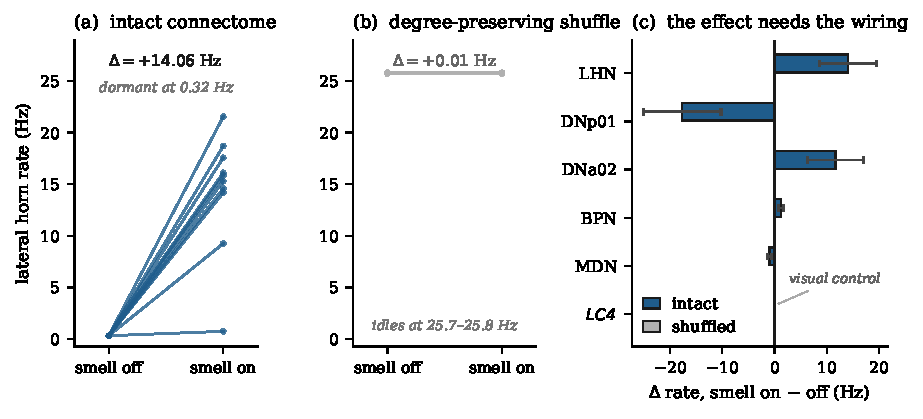
\includegraphics[width=\textwidth]{figs/fig3_olfaction.pdf}
\caption{Olfactory valence reaches the descending neurons, and needs the wiring
to do it. \textbf{(a)} Per-seed lateral horn rate with smell off and on in the
intact connectome; all ten seeds rise. \textbf{(b)} The same protocol on a
degree-preserving shuffle of the same graph: no seed moves appreciably, and the
shuffled baseline idles near 21\,Hz where the intact pathway is dormant at
0.32\,Hz. \textbf{(c)} Mean change per population, both arms (error bars are
s.d.\ over ten seeds). \cell{LC4} is a visual cell included as a control: it
should not move, and does not.}
\label{fig:olfaction}
\end{figure}

The lateral horn, the innate-valence pathway~\citep{jefferis2007,dolan2019},
is dormant at 0.32\,Hz without smell and rises to $14.1\pm5.5$\,Hz with it,
in all ten seeds (Table~\ref{tab:m8}). The effect reaches the descending
neurons in \emph{one synapse}, and its sign is predicted by the wiring:
$\cell{LH}\rightarrow\cell{DNp01}$ is $-248$ synapses, hence inhibitory, and
\cell{DNp01} is suppressed by $17.7\pm7.4$\,Hz, in nine seeds of ten.
Meanwhile \cell{LC4}, a visual population that should not move at all, does
not: it shifts by $-0.00\pm0.02$\,Hz, four orders of magnitude below the
lateral horn response it bounds.

Crucially, a degree-preserving shuffle of the same graph, run through the
identical protocol and the identical seeds, does not reproduce this
(Table~\ref{tab:m8}, right). The valence and steering effects collapse by two
to three orders of magnitude, \cell{LHN} from $+14.06$ to $+0.01$\,Hz
($1563\times$), \cell{DNa02} $102\times$, \cell{DNp01} to within noise of
zero, landing at the $0.00$--$0.11$\,Hz scale of the \cell{LC4} control, that
is,
at the network's generic coupling floor.

Sign consistency and effect magnitude discriminate differently here, and only
the second separates the arms. Sign consistency does \emph{not}: several
shuffled populations remain fairly
sign-consistent across seeds, including \cell{LC4} at $10/10$, the one
population that should not be responding at all. What discriminates is
magnitude. A sign test on a $0.01$\,Hz effect is a statement
about a systematic that is three orders of magnitude too small to matter, and
and we interpret it accordingly. The shuffled \cell{DNp01} residual
reversed sign between two independent executions of the protocol, where every
intact effect held its direction, the behaviour expected of noise rather
than of a transformation. In summary: the intact effects are large and
reproducible while the shuffled ones sit at the control's floor.
\emph{The effect requires the wiring.}

The \cell{BPN} and \cell{MDN} walking effects support a weaker claim than the
rest. They are consistent in direction across all ten seeds, but at
$\pm1$\,Hz they are only ${\sim}17\times$ above the shuffled floor rather than
${\sim}100\times$, and we draw no conclusion from them in isolation.

The shuffle also changes the baseline in an informative way. Without smell the
intact lateral horn sits at 0.32\,Hz; the shuffled one idles at
25.7--25.8\,Hz across seeds, an $80\times$ higher floor. Preserving degree
while destroying specificity does not merely
remove the response: it removes the \emph{quiet}. The intact lateral horn is
selectively silent and selectively driven, which is the behaviour a
labelled-line valence pathway should show, and neither property survives
rewiring.

Two caveats apply to this result throughout. Odour source distances are read from the
engine's label buffer, so the model was \emph{told} that enemies exist; this is
evidence about what the connectome does with a signal, not evidence that it can
detect one. And 1{,}227 lateral horn neurons pooled together mixes many
functional channels, so ``the lateral horn responds'' is coarser than it sounds.

\subsubsection*{Synaptic weight against path length}
We first routed the same odour at the \cell{pC1} aggression neurons, on the
strength of a three-hop path touching 8 of 10 cells, and it failed flat:
0.00\,Hz across a tenfold sweep of drive. Measured afterwards: the reason is
structural: \cell{DA1}'s contribution is a rounding error against \cell{pC1}'s
balanced $+530/-555$ of input, and \cell{pC1} is a bistable latch that must be
pushed over rather than nudged. The lateral horn is the opposite on every
count: it receives 21\% of the odour relay's entire output, has no latch,
and sits one hop from the output. Hop count is a poor proxy for influence in a
connectome; synaptic weight against competing input is the quantity that
matters.

\subsection{Validity of shuffle controls in closed loop}
\label{sec:shuffle}

Degree-preserving shuffles are the standard control for attributing an effect
to connectivity, and we use one above. But in a closed loop they silently stop
being a control.

We measured this directly. Over one matched episode the intact agent
encountered an enemy on 186 of 500 tics and finished at full health; the
shuffled agent encountered one on 489 of 492 tics and finished at 16 health.
The point this episode makes is qualitative, that the arms visit different
states, and it does not require the difference to be of any particular
size; but see the power note below before reading episode counts as effects. The two arms
behaved differently, and because behaviour determines what the agent sees, they
were no longer sampling the same stimulus distribution. Any cross-arm
correlation then compares two different worlds rather than two different
brains.

The consequence generalizes to any embodied connectome study: \emph{controls
must hold the stimulus fixed}, which in practice means running the comparison
open loop, as we do for the olfaction result.

\subsection{Motion vision and looming}

Direction selectivity fails. Presenting drifting gratings and measuring the
direction selectivity index
$\mathrm{DSI}=(R_{\mathrm{pref}}-R_{\mathrm{null}})/(R_{\mathrm{pref}}+R_{\mathrm{null}})$
in \cell{T4}/\cell{T5}, the canonical elementary motion
detectors~\citep{maisak2013}, gives $|\mathrm{DSI}|\leq0.0121$. Experimental
studies routinely \emph{select} terminals for analysis at $\mathrm{DSI}>0.5$,
so the model sits some $40\times$ below the threshold at which a real
terminal would merely qualify as direction-tuned.

Looming fails in the same way and more starkly (Table~\ref{tab:looming}).
Neither the intact nor a degree-preserving shuffled connectome distinguishes an
expanding from a contracting stimulus; both instead show
$\text{static}\gg\text{looming}\approx\text{receding}$, the signature of a
response to dark \emph{area} rather than to expansion. Because the shuffled
graph performs comparably: the measurable looming response is not attributable
to connectivity at all.

\begin{table}[t]\centering\small
\caption{Looming (M4), open loop, mean rate in Hz. Neither arm separates
looming from receding, and the intact connectome does not outperform a
degree-preserving shuffle.}
\label{tab:looming}
\begin{tabular}{lrrr@{\hskip 2em}rrr}
\toprule
& \multicolumn{3}{c}{\bf Intact} & \multicolumn{3}{c}{\bf Shuffled}\\
\cmidrule(r){2-4}\cmidrule(l){5-7}
& \cell{LC4} & \cell{LPLC2} & \cell{DNp01} & \cell{LC4} & \cell{LPLC2} & \cell{DNp01}\\
\midrule
Looming  & 36.06 & 0.00 & 139.0 & 7.04 & 2.82 & 88.7\\
Static   & 73.37 & 0.02 & 149.3 & 45.15 & 14.41 & 207.0\\
Receding & 34.58 & 0.00 & 149.7 & 6.19 & 2.50 & 84.0\\
\bottomrule
\end{tabular}
\end{table}

\subsubsection*{State of the looming detector}
In closed loop \cell{LPLC2} reads exactly $0.00$\,Hz, and the reason is
measurable. It sits at $-52.2$\,mV, \emph{below} its own resting potential
and $7.2$\,mV from threshold, because its heaviest input, \cell{PVLP011} at
$-45.6$ synapses per cell, fires at 371\,Hz. The model's absolute refractory
ceiling is $1/t_{\mathrm{refrac}}=455$\,Hz, so that one inhibitory cell runs at
82\% of the maximum rate the model permits, and the inhibitory conductance it
delivers exceeds the excitatory arm (\cell{Tm5f}, $+44.7$ synapses per cell but
only 36\,Hz) by roughly tenfold. This is the \cell{T4a} arm imbalance again, in
a second and independent circuit.

That it is an imbalance rather than a shortage is what makes it diagnostic. We
swept every input-side scale available (photoreceptor drive, the graded rate
ceiling, and Weber contrast gain) and \cell{LPLC2} does not leave $0.00$\,Hz
at any setting. Reducing drive lowers \cell{PVLP011} from 371 to 113\,Hz but
takes \cell{LC4} from 53 to $0.0$\,Hz with it. The result is expected on
inspection: an input scale multiplies both arms of a ratio and cancels, so no
common gain can change a $10\!:\!1$ imbalance. Only a gain that acts
differentially on the two arms can, which is to say a per-type gain: the
quantity the connectome does not specify and the optimized model of
\citet{lappalainen2024} obtains by fitting.

A tonic depolarising drive to the optic lobe does release it, and shows the
same trade rather than escaping it. Raising the bias from 0 to 6\,mV lifts
\cell{LPLC2} from $0.0$ to $64.7$\,Hz, but it also lifts \cell{MDN}, and the
walking command is $\cell{BPN}-\cell{MDN}$: that difference falls from
$+22$\,Hz to $+0.3$\,Hz by 2\,mV and reverses sign by 6\,mV, at which point the
model walks backwards. Meanwhile the population above 200\,Hz grows from 197
cells to 991. There is no setting at which the looming pathway conducts and
locomotion survives.

A blank-field control shows the trade is worse than that, and it is the reason
we report bias sweeps with one. Presenting an \emph{empty screen} at
7.5\,mV bias drives \cell{LPLC2} to 76.17\,Hz, against 76.22\,Hz for an
expanding disc, a stimulus contribution of 0.07\%. At 4\,mV it is 30.52 blank
against 30.62 looming. The bias that releases the cell is the same quantity that
determines its output: past threshold we are no longer measuring vision but
measuring the bias, and the fraction of the response attributable to the picture
\emph{falls} as the bias rises. There are two regimes and neither is looming
detection: \cell{LPLC2} silent, or \cell{LPLC2} firing at a rate the stimulus
barely perturbs. Reporting the looming response alone, without the blank, would
have made 76\,Hz look like success.

We also tested whether the failure is an artefact of where visual drive enters.
By default we inject at the lamina monopolars, one synapse past the
photoreceptors, which bypasses two real features of the eye: neural
superposition, in which six photoreceptors sharing a visual direction converge
on one cartridge, and the histaminergic first synapse that inverts the signal.
Injecting at \cell{R1-6} instead restores both. It changes nothing. At matched
bias the two sites agree to within the blank-field offset (\cell{LPLC2} 18.4
against 30.6 at 4\,mV, 76.2 against 76.4 at 7.5\,mV), and at zero bias
photoreceptor injection is silent throughout, because the inhibition-dominated
optic lobe has no baseline to disinhibit from. The one thing photoreceptor
injection does carry is a bias of its own: FAFB's uneven optic-lobe
proofreading recovers a column for 451 of 785 left columns against 749 of 796
right, so it is unusable for any measurement of a left--right difference, which
is why the default sits at the lamina.

Across every condition in that sweep, looming and receding differ by less than
the blank-field offset, and the \emph{sign} of the difference flips between
conditions. The only regime with genuine stimulus-driven structure is zero bias
at the lamina, where \cell{LC4} gives 77.2\,Hz for a static disc against
24.9\,Hz blank, a real threefold response, to dark \emph{area}. The model
reports how much dark is present, never whether it is growing.

Downstream visual functions fail correspondingly. \cell{LPLC2} activity is
uncorrelated with true angular size ($r=+0.000$), and no azimuth signal exists
anywhere we could find: neither \cell{LC11} ($r=+0.034$) nor \cell{LC4}
($r=+0.070$) carries target bearing. \cell{LC10a}, the cell type that would
carry it, is silent at 0.00\,Hz, receiving only $+45/-83$ synapses per cell
against \cell{LC11}'s $+477/-456$ and \cell{LC4}'s $+439/-259$; it is held down
by \cell{AOTU042} and \cell{TuTuAa}. Its known state-dependent gain boost is a
\emph{male} courtship mechanism gated by \cell{P1}, and FAFB is a female brain,
so that circuit is absent. Nor is there a state signal to substitute for it.
\cell{AOTU042} suppresses
\cell{LC10a} at $-18$ synapses per cell, but \cell{pC1} and \cell{AOTU042} are
not connected in this brain at all, zero edges in either direction, at any
synapse threshold, so the aggression state cannot reach that suppression to
lift it or to deepen it.

\subsection{Candidate mechanisms for the motion failure}
\label{sec:mech}

\begin{figure}[t]\centering
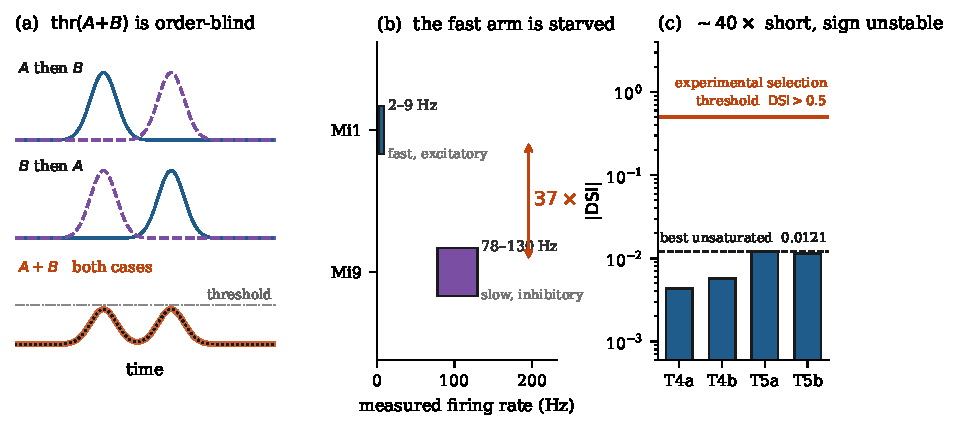
\includegraphics[width=\textwidth]{figs/fig2_mechanism.pdf}
\caption{The motion failure. \textbf{(a)} The order-blindness argument we
withdraw: for a \emph{memoryless} unit, ``$A$ then $B$'' and ``$B$ then $A$''
produce identical sums (rust curve, second case overlaid dotted), so a
threshold on that sum responds identically. This panel does not describe the
present model, whose conduction delays and synaptic time constants make the
summation history-dependent; a correlator built from the same units reaches
$\mathrm{DSI}=-0.79$ (Sec.~\ref{sec:mech}). \textbf{(b)} Measured firing
rates of \cell{T4a}'s two correlator arms: the fast excitatory arm
(\cell{Mi1}) is suppressed by glutamatergic \cell{L1} while the slow inhibitory
arm (\cell{Mi9}) runs freely, a $37\times$ conductance imbalance.
\textbf{(c)} Resulting direction selectivity with graded optic-lobe units.
Magnitudes fall some $40\times$ short of the value at which experimental
studies merely \emph{select} a terminal as direction-tuned, and across 45
unsaturated operating points the two mirror pairs oppose at only 3, which is
below chance: the sign is fluctuating, not small-but-real.}
\label{fig:mechanism}
\end{figure}

Direction selectivity and looming selectivity are both computations over the
\emph{temporal order} in which neighbouring retinotopic columns activate.
Motion to the right makes column $A$ lead column $B$; motion to the left makes
$B$ lead $A$. The two cases contain identical events and differ only in order.

A symmetry argument appears to make the failure structural. Presynaptic inputs
sum into a conductance and the only nonlinearity is a threshold on that sum;
since $\mathrm{thr}(A+B)$ is symmetric in its arguments, no unit of this class
would distinguish the two cases. The argument is invalid, because it holds only
for a unit with no memory. The model has memory in two places the argument
ignores: per-connection conduction delays, and a synaptic conductance that
decays with $\tau_{\mathrm{syn}}=5$\,ms rather than vanishing within the step.
A delayed arm and a persistent conductance make the summand at any instant
depend on stimulus history, and the symmetry does not hold.

We settled this by construction rather than by argument. Using the same neuron
model, the same integrator and the same time step, we built a two-input
correlator (two input units, one delayed, converging on a third) and
measured it under the identical grating protocol. It reaches
$\mathrm{DSI}=-0.79\pm0.017$ (30\,s $\times$ 5 seeds), against
$0.002$--$0.016$ for \cell{T4a} in the network. The model class can compute
direction selectivity to a magnitude far above the experimental selection
threshold. Whatever prevents the network from doing so, it is not the
arithmetic of summation and threshold. Biological elementary motion detectors
combine a delayed and an undelayed arm
\emph{multiplicatively}~\citep{hassenstein1956,borst2010}, realized in
\emph{Drosophila} as preferred-direction enhancement together with
null-direction suppression~\citep{haag2016,gruntman2018}; a delay plus a
saturating threshold approximates that product well enough to yield the
$0.79$ above.

Both ingredients are present in the graph, and we verified them. \cell{T4a}
receives fast centred excitation (\cell{Mi1} $+30.6$, \cell{Tm3} $+7.0$) and
slow flanking inhibition on opposite sides (\cell{Mi9} $-7.4$ at
$(-0.76,+0.26)$; \cell{Mi4} $-3.4$ at $(+0.39,-0.60)$), with four subtypes on
four mirrored axes. The stimulus reaches them: \cell{L1}'s response phase
advances at $-20.0$\,deg/deg against an expected $20.0$, and this retinotopic
travelling wave survives to \cell{T4a}.

We implemented and measured six candidate remedies. Five produced nothing:
per-type conduction delays (1.8--240\,ms), per-neuron membrane time constants
(5--200\,ms), conductance-based shunting synapses, a forced high-conductance
state ($g_{\mathrm{tot}}=105$, two orders of magnitude past the linear regime),
and population pooling (per-cell DSI against per-cell input offset, $r=+0.043$
over 874 cells). The sixth, modelling the optic lobe as \emph{graded,
non-spiking} units, which is what photoreceptors and lamina monopolar cells
actually are, was the only one to produce a measurable effect at all
(Table~\ref{tab:dsi}), and it is small enough that its sign has to be checked
rather than assumed.

Checking it requires sweeping the operating point rather than picking one,
because the dominant influence on the number is not the wiring: graded units
are capped at 200\,Hz, and a unit against its ceiling reports
$\mathrm{DSI}\approx0$ whatever its inputs do. We therefore swept bias, spatial
period and temporal frequency (72 points), kept the 45 below 75\% saturation,
and report the largest effect among them. Two things follow. The magnitude is
$|\mathrm{DSI}|\leq0.0121$, some $40\times$ below the value at which
experimental studies merely \emph{select} a terminal as direction-tuned. And
the qualitative signature is absent: both mirror pairs oppose at only 3 of the
45 unsaturated points, where two independent coin flips would give about 11. A
correlator's sign does not depend on its operating point, so what we are
measuring is a quantity fluctuating about zero rather than a small but real
selectivity. Individual configurations can show apparent mirror opposition, but it does not
survive the sweep.

\begin{table}[t]\centering\small
\caption{Direction selectivity, at the strongest operating point that is not
saturated. Graded units are capped at 200\,Hz and a
unit against its ceiling reports $\mathrm{DSI}\approx0$ whatever its inputs
do, so we sweep bias, spatial period and temporal frequency
(72 points), keep the 45 below
75\% saturation, and report the largest
effect among them --- bias 1.0\,mV, period
30$^\circ$, 1\,Hz. The magnitude is
$41\times$ below the value at which experimental
studies merely \emph{select} a terminal as direction-tuned. The sign is not
reliable either: both mirror pairs oppose at only 3 of
45 unsaturated points (7\%), by pair \cell{T4a/T4b} 5/45, \cell{T5a/T5b} 15/45. A
correlator's sign should not depend on the operating point, so this is a
quantity fluctuating about zero rather than a small but real selectivity.}
\label{tab:dsi}
\begin{tabular}{lrrl}
\toprule
Pathway & \multicolumn{2}{c}{DSI} & Mirror pair\\
\midrule
ON  & \cell{T4a} $-0.00431$ & \cell{T4b} $-0.00570$ & same sign\\
OFF & \cell{T5a} $-0.01208$ & \cell{T5b} $-0.01147$ & same sign\\
\bottomrule
\end{tabular}
\end{table}


One imbalance is measurable and specific, though the tests below show it is
not sufficient to explain the failure: the fast arm is starved.
Weighting \cell{T4a}'s inputs by measured firing rate rather than synapse count
gives excitation 189 against inhibition 558, a $3.0\times$ imbalance in drive;
the realised synaptic conductances are $g_e=0.0018$ against $g_i=0.0667$, a
ratio of $37\times$. The two quantities measure different things,
rate-weighted input against the conductance it actually produces, and it is
the second that sets how far the excitatory arm can move the membrane.
\cell{Mi1} sits at 2--9\,Hz because \cell{L1} suppresses it ($-77.3$,
glutamatergic and therefore inhibitory), while \cell{Mi9} runs at
78--130\,Hz. The ON pathway is disinhibitory and, with uniform per-type gains,
never rebalances. The OFF pathway, which does not depend on that
disinhibition, conducts normally (\cell{T5a} 58\,Hz against \cell{T4a} 2\,Hz),
an internal control indicating the deficit is pathway-specific rather than
a global failure of the optic lobe.

Correcting that imbalance does not rescue selectivity. We rebalanced the arms
two ways: presynaptic short-term depression (Tsodyks--Markram, $U=0.3$,
$\tau_{\mathrm{rec}}=0.5$\,s), which depresses the tonically active inhibitory
arm more than the sparsely active excitatory one; and transplanting the
per-type gains of the optimized model of \citet{lappalainen2024} onto the
matching connections (571 of its 604 type-pairs align with our graph). Both
\emph{lowered} $|\mathrm{DSI}|$. The $37\times$ ratio is therefore a real
property of the wiring under a single global gain, but it is not the operative
cause, and the hypothesis drawn from it, that optimization
supplies relative gain along the ON pathway's disinhibitory chain, is not
supported by the transplant. We note the transplant is approximate: that model
was fitted on a different reconstruction (fib25--fib19), so an unmatched gain
is not evidence against the hypothesis, only against the simplest version of
it.

Two further explanations were tested after the analysis above and are
reported here because they are the two that a reader would reach for next.

\emph{The competing-input hypothesis.} If the correlator is present but
swamped, removing everything else should reveal it. We tested this in the
RUNNING network rather than by isolated replay, which the caution at the end of
this section explains cannot be trusted. Silencing every input onto
\cell{T4a}/\cell{T4b} except \cell{Mi1} and \cell{Mi9}, 14{,}594 of
24{,}944 edges, does not raise selectivity: over the 45 operating points
unsaturated in both conditions, $\max|\mathrm{DSI}|$ moves from $0.0057$ to
$0.0020$. Adding back \cell{Tm3}, \cell{Mi4} or \cell{CT1} individually gives
$0.0035$, $0.0021$ and $0.0034$. \cell{T5a}/\cell{T5b} are never ablated and
serve as a within-run control: their mean $|\mathrm{DSI}|$ is
$0.00442$--$0.00444$ in all five conditions, so nothing leaked. The
manipulation is electrically real: \cell{T4a}'s rate ranges 63 to 97\,Hz
across conditions. The correlator fails even when it is the only thing
connected.

\emph{Dendritic compartmentalization.} A point neuron makes every synapse
electrically identical, so a shunt divides the whole cell, whereas
null-direction suppression is local to a branch. We split all 11{,}822
\cell{T4}/\cell{T5} into a spiking soma and a passive dendrite coupled by an
axial conductance, assigning each input by retinotopy alone: same column to
the soma, different column to the dendrite. The rule reproduces the anatomy
without naming a cell type (\cell{Mi9} 97\% distal, \cell{Mi4} 98\%) and is
electrically effective (rates fall $193\to151$\,Hz; unsaturated points rise
$45\to63$). It does not rescue selectivity: $\max|\mathrm{DSI}|$
$0.0121\to0.0128$, mirror-pair sign below chance throughout. Two compartments
cannot represent the ordering of arms along a real \cell{T4} dendrite, which
is the obvious next refinement.

A related measurement bounds where the failure cannot be. At the tonic bias of
7.5\,mV that makes an inhibition-dominated circuit conduct, the arms carry
almost no time-varying signal at all: \cell{Tm3} and \cell{Mi4} sit at their
ceiling 94.7\% and 75.6\% of the time with modulation amplitude $0.000$\,Hz,
and \cell{Mi9} delivers $0.93$\,Hz out of a 200\,Hz range. A correlator has
nothing to correlate there. The operating-point sweep already excludes that
regime, its filter removes every point above 3\,mV, but the filter tests
\cell{T4}'s own saturation, not its inputs', and those are different
questions. Within the surviving range the two move together: as bias falls
from 3.0 to 1.0\,mV, arm modulation rises and $\max|\mathrm{DSI}|$ rises with
it, $0.0073\to0.0121$.

That trend does not extrapolate, and the way it fails is worth recording
because it is a trap in the measure itself. Extending the sweep below the
range previously tested, down to zero tonic drive, $\max|\mathrm{DSI}|$ keeps
rising, to $0.0164$. It is not signal. \cell{T4a} fires 2.0\,Hz there, and
the quantity a correlator actually delivers, the rate DIFFERENCE between
preferred and null, falls over the same interval, from $0.31$\,Hz at
0.75\,mV to $0.060$\,Hz at zero. The ratio grows because its denominator
collapses faster than its numerator. The mirror-pair sign agrees: across
these points the pairs share a sign on 78\% of them, where a correlator
requires opposition and chance would give 50\%. $\mathrm{DSI}$ is therefore
interpretable only in a middle band: bounded above by saturation, which the
sweep already controls, and below by the vanishing denominator, which it did
not. We report the bounded figure, $|\mathrm{DSI}|\leq0.0121$, rather than the
larger and emptier one.

What remains is a negative result without a mechanism, and we report it as
such. Nineteen candidate explanations were measured and eliminated: pooling
artefact (per-cell $r=+0.043$ over 874 cells); arm imbalance, by depression and
by gain transplant; input dilution (the correlator supplies 80--86\% of
\cell{T4a}'s input); unmodulated arms (\cell{Mi1} modulates at 125\% and
\cell{Mi9} at 89\% of their means); \cell{CT1} saturation (12{,}601 edges
ablated, no change); absent phase offset (measured mean $154^\circ$ between
arms); smeared spatial sampling (inter-column coherence $1.000$); same-column
sampling (\cell{Mi9}/\cell{Mi4} sample one column away, $1.5\%$ overlap);
opposite-flank cancellation (flanks at $139^\circ$; ablating one does not
help); graded versus spiking units; tonic bias 0--7.5\,mV; global optic-lobe
gain $\times1$--$32$; gain targeted onto \cell{T4}/\cell{T5} $\times2$--$20$;
operating point, where the isolated correlator's monotonic
DSI-versus-rate curve does not reproduce in the network; the competing-input
hypothesis, by in-network ablation; and dendritic compartmentalization. The geometry, the
delays, the phase offset and the modulation are all present and measured; the
selectivity is not. Each of these interventions addresses a component that is
not defective, which is why none of them helps. The operative cause lies in how
the components are combined, and is identified in Sec.~\ref{sec:shunt}.

Two properties of the model, rather than of the connectome, account for a
large part of the deficit, and both were found by building a correlator that
works and then adding \cell{T4}'s properties to it one at a time.

\emph{The cell is below threshold on its own inputs.} Summed over the graph,
\cell{T4a} receives $46.8$ units of excitation and $41.5$ of inhibition per
cell. Calibrating the same units in isolation, a target driven at the graded
ceiling emits nothing at a weight of $30$ and $24$\,Hz at $60$: the threshold
for any output at all falls at roughly $40$--$50$. Supplying the hand-built
correlator with \cell{T4a}'s measured weights therefore leaves it \emph{silent},
$R_{\mathrm{pref}}=R_{\mathrm{null}}=0$. Under a single global $W_{\mathrm{syn}}$
calibrated on the SEZ taste circuit, the cell can only be made to fire by the
tonic bias, which carries no stimulus information, so the selectivity we have
been measuring is a ripple on an uninformative pedestal. \cell{T5a}, at $58.9$
against $31.3$, clears the same bar, and reads $3.7\times$ the selectivity.

\emph{The graded transfer function removes the required nonlinearity.} A
correlator converts a phase difference between its arms into a rate difference,
which requires an expansive nonlinearity. A graded unit emits
$\mathrm{clamp}((v-V_{\mathrm{rest}})/\Delta,0,1)$, a \emph{linear} ramp between
its clamps. Holding the recorded \cell{Mi1}/\cell{Mi9} traces, the weights and
the delays fixed and changing only the target's transfer function gives
$\mathrm{DSI}=-0.1781$ spiking against $-0.0168$ graded, a $10.6\times$ loss;
the latter is the value the intact network reports. Modelling the optic lobe as
graded is correct for photoreceptors and lamina monopolars and was adopted for
that reason, but applied to \cell{T4} it removes the operation the cell exists
to perform.

Correcting both, spiking \cell{T4}/\cell{T5}, and optic-lobe gain in place of
the tonic bias, raises the fraction of cells above the experimental selection
threshold from $2.8\%$ to $12.3\%$. It does not produce direction selectivity.
The preferred direction remains set by the stimulus rather than by the wiring:
across six spatial period and temporal frequency combinations, the fraction of
\cell{T5a} cells preferring one direction swings from $34\%$ to $70\%$, crossing
and reversing, and the residual response shows no delay tuning at all: varying
the slow arm from $20$ to $160$\,ms moves the directional signal only between
$1.04$ and $1.29$\,Hz. A correlator's preference is a property of its geometry
and cannot depend on the stimulus that probes it. We therefore do not describe
the residual as weak direction selectivity; it is a stimulus-timing artefact,
which also explains the below-chance mirror opposition reported above.

One methodological result follows from this work: isolated replay is not a
valid control for this question. Driving \cell{T4a} cells with their own
recorded inputs in isolation yields mean $|\mathrm{DSI}|=0.37$, which invites a
causal account. The same procedure applied to a \emph{single} input, where the
geometry makes direction selectivity impossible, returns $0.12$ rather than the
required $0$. The cause is that \cell{Mi1} is itself weakly selective
($|\mathrm{DSI}|=0.040$) and a threshold unit amplifies that residue. Isolated
replay is not a clean control for this question.

\subsection{Cancellation of the shunting nonlinearity}
\label{sec:shunt}

Direction selectivity requires a multiplicative interaction between the two
correlator arms. In a conductance-based neuron the only available source of
that interaction is inhibitory division: the membrane relaxes toward
$v_\infty = (V_{\mathrm{rest}} + g_e E_e + g_i E_i)/(1 + g_e + g_i)$, so
inhibition divides rather than subtracts.

Measurement at the operating point shows the division is cancelled by its own
consequence. Inhibition raises $g_{\mathrm{tot}}$ from $2.21$ to $3.92$, a
factor of $1.77$, and simultaneously lowers $v_\infty$ from $-23.5$ to
$-43.4$\,mV, which raises the excitatory driving force $(E_e - v)$ by a factor
of $1.85$. The net interaction is $1.85/1.77 = 1.056$. Across \cell{T4a},
\cell{T4b}, \cell{T5a} and \cell{T5b} the interaction does not exceed $11\%$,
and its sign is inverted: inhibition slightly increases excitatory gain. Fitting
the realised conductance trajectory confirms this independently. A purely
additive model $v = a + b\,g_e + c\,g_i$ accounts for $R^2 = 0.865$ of
\cell{T4a}'s membrane voltage, and adding the bilinear term $g_e g_i$ increases
this by $2.2$ percentage points.

The cell therefore sums its inputs. Summation is symmetric in its arguments and
cannot recover temporal order at any wiring, which accounts for the failure of
the nineteen candidate remedies listed above: each addressed a component that
was not defective.

The interaction is governed by $g_i/g_e$ rather than by $g_{\mathrm{tot}}$.
When the two conductances are comparable, the driving-force term cancels the
shunt; the division survives only when inhibition substantially exceeds
excitation.

\subsection{Comparison of conductance parameterisations}
\label{sec:threeway}

The preceding result makes the assignment of synaptic conductances the
study's operative variable. We compare three ways of setting it, together with
the uniform scaling that motivates the third.

\begin{table}[t]\centering
\small
\begin{tabular}{llrrll}
\toprule
parameterisation & values from & proj.\ DSI & behav. & gustatory & olfactory\\
\midrule
(i) single global gain & fitted on taste & $-0.0107$ & 0/18 & pass & pass\\
(ii) per-receptor, global & published physiology & $-0.0356$ & n/a & pass$^{*}$ & \textbf{fail}\\
(iii) uniform $\times2$, global & search & $-0.0533$ & n/a & \textbf{fail} & n/a\\
(iv) $\times2$ on vision only & search & $\mathbf{-0.0716}$ & \textbf{10/18} & pass & pass\\
\bottomrule
\end{tabular}
\caption{Parameterisations of synaptic conductance. Projected DSI is the
population mean after projecting each cell's response onto its own correlator
axis; the raw population mean cancels across cells whose axes oppose.
Behavioural column gives the number of eighteen metrics on which the model
separates from a command-matched control over thirty held-out environment
seeds. Row (iii) fails because bitter stimulation drives the proboscis motor
pool to $168$\,Hz instead of suppressing it. Row (ii) passes the gustatory
checks but degraded ($^{*}$sugar $63.79\pm9.31$ against $73.58\pm1.44$\,Hz,
suppression $95\%$ against $99\%$) and fails olfaction. Both global
assignments break a circuit the frozen model preserves; only the regional
assignment does not.}
\label{tab:threeway}
\end{table}

\emph{(i) A single global gain.} This is the frozen model. Direction
selectivity is $40\times$ below the experimental selection threshold and the
model does not separate from the control on any behavioural measure.

\emph{(ii) Per-receptor conductances from published physiology.} Neither value
was chosen with reference to any result reported here. GABAergic conductance is
$2.5\times$ cholinergic in two unrelated preparations: \citet{suodowd2003}
record quantal events for both transmitters in the same cells, and
\citet{groschner2022} fit adult \cell{T4} in vivo. We take
$g_{\mathrm{GluCl}}/g_{\mathrm{ACh}} = 0.92$ from the latter and note that it is
a fit rather than a measurement, no direct \emph{Drosophila} GluCl conductance
having been published. Applying both ratios raises $g_i/g_e$ from $0.713$ to
$1.323$ and improves selectivity $3.3\times$, with the absolute rate difference
rising from $1.09$ to $2.97$\,Hz. It nonetheless fails the olfactory
constraint. \cell{DNp01} falls to $0.00$\,Hz in both the odour and control
arms: raising inhibition brain-wide silences the neuron outright, so no
baseline discharge remains for the odour to suppress and the measured
difference is zero by construction rather than by loss of the pathway.
\cell{LHN} falls from $+14.38$ to $+4.16$\,Hz and \cell{DNa02} from $+12.12$
to $+0.05$\,Hz. This is the informative result in the comparison. The values
are not ours and were not selected to produce any outcome reported here, yet
applying them uniformly breaks a circuit that the cruder single-gain model
preserves. Correct per-receptor ratios are therefore necessary but not
sufficient: the assignment must also be regional, which is a property of this
brain that receptor measurements cannot themselves supply.

\emph{(iii) Uniform scaling, applied globally.} Doubling every inhibitory
synapse improves selectivity but inverts the gustatory response: bitter
stimulation drives the proboscis motor pool at $168$\,Hz instead of suppressing
it, and the dose-response relation degrades to noise. The inversion occurs
because $557{,}080$ of $1{,}099{,}675$ inhibitory edges ($51\%$) terminate on
inhibitory neurons, so uniform scaling amplifies disinhibition equally and the
sign of the circuit reverses.

\emph{(iv) The same factor restricted to the visual populations.} The gustatory
result is numerically unchanged to the reported precision (sugar
$73.58\pm1.44$\,Hz, bitter $0.00$, $99\%$ suppression, six of six acceptance
checks), because \cell{MN9} receives $0.00\%$ of its input synapses from the
scaled populations and a regional parameter has no path into the circuit.
Olfaction is preserved, including the readout that is structurally exposed:
\cell{DNp01} draws $20.5\%$ of its input from the scaled populations and holds
at $-17.02\pm7.15$\,Hz against a baseline of $-18.13\pm2.48$\,Hz. The one cost
is \cell{DNa02}, which falls from $12.12$ to $2.65$\,Hz.

Rows (iii) and (iv) differ only in the region to which an identical factor is
applied. The comparison establishes that a single global synaptic gain is not
merely an approximation but an inconsistency: the optic lobe requires a
conductance ratio the subesophageal zone does not tolerate. \citet{groschner2022}
report inhibitory-to-excitatory conductance ratios of $7.7$ and $10.9$ in adult
lobula plate neurons, so the factor of two used here is conservative relative to
the published requirement.

\subsection{Closed-loop behaviour}
\label{sec:behaviour}

Configuration (iv) was evaluated against the command-matched AR(1) control on
thirty environment seeds not used while selecting parameters.

\begin{center}
\small
\begin{tabular}{lrr}
\toprule
paired difference vs.\ control & regional (iv) & frozen (i)\\
\midrule
tiles visited            & $+9.7\pm3.8$    & $-1.0\pm3.4$\\
collisions per 1k tics   & $-4.88\pm1.9$   & $-0.5\pm3.6$\\
stuck fraction           & $-0.13\pm0.0$   & $+0.02\pm0.1$\\
path length              & $+511\pm230$    & $-127\pm195$\\
health collected         & $+11.9\pm10.8$  & $-7.7\pm10.4$\\
vision--steering $r$     & $-0.18$         & $-0.04$\\
\bottomrule
\end{tabular}
\end{center}

Ten of eighteen metrics separate from the control under (iv) and none under
(i). In absolute terms the regional model collects $30.0$ health units against
its matched control's $18.1$, where the frozen model collects $13.2$ against
$20.9$.

Three controls exclude the possibility that the effect follows from reduced
drive alone. Matching the firing rate by lowering gain instead of raising
inhibition yields $-0.0152$ against $-0.0716$. Applying the identical factor to
non-visual inhibitory synapses yields $-0.0102$ against an unmanipulated
$-0.0107$. On the $1{,}869$ cells driven above threshold in both conditions,
projected selectivity moves from $+0.0001$ to $-0.0720$, excluding selection
among a shrinking population.

Two further controls bound the result. With the retina frozen on a single
frame, the collision advantage remains significant ($-3.56\pm2.9$), indicating
that approximately half of it derives from the temporal structure of the motor
command rather than from vision. Mirroring the retina reverses the
vision--steering correlation as expected ($-0.21$ to $+0.13$) but reduces the
behavioural point estimates by a factor of three rather than abolishing them.
We initially described the optimum as narrow, on the grounds that selectivity
collapses at a scaling of four. A structured search over $137$ parameter
combinations measured the local curvature directly and does not support that
reading. Holding the score within $20\%$ of its maximum admits scalings from
$1.67$ to $2.81$, a band $\pm25\%$ about the chosen value on a three-stimulus
mean; the collapse at four is the far shoulder rather than the local shape.
That search found no feasible configuration superior to (iv). A scaling of
$2.5$ raises the ratio further but not the absolute rate difference, which is
maximal at $2.0$ ($3.97$\,Hz averaged over three stimuli) and reverses on both
held-out stimuli. Scaling the complementary non-visual population has no effect
at any value between $0.5$ and $3$, despite rescaling $467{,}082$ edges, which
is a further specificity control. Every higher-scoring point the search located
lay outside the feasible region, failing the olfactory constraint in the manner
described for row (ii).

\section{Discussion}

The dissociation we observe is not between easy and hard computations, nor
between small and large circuits. It is between computations that a linear
summation followed by a threshold can express and those it cannot. Gustatory
and innate-olfactory valence are, at the level the connectome constrains them,
weighted sums with signs: sugar excites a motor pool, bitter inhibits it, an
odour drives a valence region that inhibits an escape neuron. Those transfer.
Motion direction is a product of a delayed and an undelayed signal, and it does
not.

This result is easily over-read as a claim about connectomics, and we state its
scope precisely. The connectome contains the correlator: the geometry, the
mirrored axes, the phase offset and the travelling wave that drives them are all
present and measured. What the frozen model fails to supply is the arithmetic
that combines them. A product requires a nonlinear interaction between the arms,
which in a conductance-based neuron can only come from inhibitory division, and
that division is cancelled by the hyperpolarisation it produces
(Sec.~\ref{sec:shunt}). The cell sums where it must multiply. This accounts for
the twenty candidate remedies that changed nothing: each addressed a component
that was not defective. It also accounts for the one remedy that appeared
promising and was not, the $37\times$ imbalance between the arms, which is a
real property of the wiring but not the operative cause, since correcting it by
short-term depression and by transplanting an optimized model's gains both
lowered selectivity.

Restoring the interaction requires raising the inhibitory-to-excitatory
conductance ratio, and the constraint that emerges is the paper's substantive
claim. No single value serves the whole brain. The optic lobe requires a ratio
that inverts the gustatory circuit, because $51\%$ of inhibitory synapses
terminate on inhibitory neurons and uniform scaling amplifies disinhibition
equally. The same factor applied regionally leaves the gustatory circuit
numerically unchanged. A single global synaptic gain is therefore not an
approximation to be refined but an assumption that cannot hold, and the
connectome is silent on the point: synapse counts constrain relative weights
within a target, not the conductance scale across regions.

Placed beside \citet{lappalainen2024} this is informative rather than merely
negative. That model shares our wiring and recovers motion selectivity by
optimizing its unknown parameters, where ours fixes them to a single published
value. The difference between the outcomes measures what optimization supplies.
Transplanting its per-type gains directly does not transfer the benefit, so
what it supplies is not gain as a lookup table; the regional result suggests it
is at least in part the freedom for conductance scale to differ between
circuits, which per-type parameters express implicitly. Published physiology is
consistent with this reading, reporting GABAergic conductances around
$2.5\times$ cholinergic and inhibitory-to-excitatory ratios of $7.7$ and $10.9$
in adult lobula plate neurons \citep{suodowd2003,groschner2022}. Applying those
measured ratios uniformly, however, is not sufficient: it improves selectivity
and breaks olfaction (Table~\ref{tab:threeway}), which indicates that correct
per-receptor values and regional assignment are separate requirements.

The behavioural result should be read with its controls. Ten of eighteen
measures separate from a command-matched control on held-out seeds where the
frozen model separates on none, and the vision-steering correlation moves from
$-0.04$ to $-0.18$. With the retina frozen, however, roughly half the collision
advantage remains, so a substantial fraction reflects the temporal structure of
the motor command rather than vision, and mirroring the retina reduces the
behavioural estimates threefold rather than abolishing them. Selectivity also
remains an order of magnitude below the experimental selection threshold. The
defensible claim is that removing an identified obstacle produces measurable
closed-loop behaviour, not that the model sees motion as a fly does.

Two further readings should be excluded. First, none of this is a claim about
whether a fly brain can play a video game. The environment lies outside the
animal's evolutionary experience and the model has no ventral nerve cord, so
the behavioural measures are used as a sensitive assay of whether a
sensorimotor transformation is present at all, not as a measure of competence. Second: the olfaction result
is not evidence of enemy detection: the odour magnitude is supplied by the
engine. What both results measure is transfer: whether a transformation
implied by the wiring appears in a running system.

\subsection{Limitations}

\begin{itemize}\itemsep2pt
\item \textbf{No ventral nerve cord.} FAFB is brain-only, so the game's
movement code substitutes for legs. All behavioural \emph{timescales} are the
engine's; claims are restricted to descending-neuron activity.
\item \textbf{No gap junctions.} EM reconstruction captures chemical synapses;
the giant fibre's fastest output is electrical and therefore invisible here.
\item \textbf{No neuromodulation.} Dopamine, octopamine and serotonin are
flattened to fast excitation.
\item \textbf{$n=1$ brain, and its halves are not mirror images.} \cell{DNa02}
sits ${\sim}2\times$ higher on the right than the left, which is a standing turn
command until removed by a slow baseline.
\item \textbf{Angular scale is calibrated, not measured.} The lattice is real
but its axes are not isotropic in visual angle, so each is scaled to the
published field of view. Absolute angular claims inherit this.
\item \textbf{The gustatory control is partly true by construction}, since
$W_{\mathrm{syn}}$ is fitted on it.
\item \textbf{Single stimulus environment.} All visual results come from one
rendering engine with one viewport geometry; we have not tested whether a
different visual statistic changes the arm imbalance.
\end{itemize}

\section{Methods}

\subsection{Connectome data}

The connectome is FlyWire FAFB v783~\citep{dorkenwald2024,schlegel2024}, frozen
October 2023. Connectivity from the Buhmann synapse
pipeline~\citep{buhmann2021} with transmitter predictions
from~\citet{eckstein2024}. Edges thresholded at five synapses. Cell types from
the consolidated typing table; \cell{BPN} and \cell{aIPg} exist only in the
free-text community label file. The data are CC BY-NC 4.0 and are not
redistributed with our code.

\subsection{Neuron model}

Neurons are leaky integrate-and-fire with the parameters listed in
Sec.~\ref{sec:model}. The subthreshold system
$\tau\,\dot v=(V_{\mathrm{rest}}-v)+g$, with $g$ decaying at
$\tau_{\mathrm{syn}}$, is integrated exactly:
\[
v(t{+}dt) = v_0 A + g_0 B + g_{\mathrm{ext}}(1-A),\qquad
A=e^{-dt/\tau_{\mathrm{mem}}},\quad
B=\tfrac{\tau_{\mathrm{syn}}}{\tau_{\mathrm{syn}}-\tau_{\mathrm{mem}}}
\bigl(e^{-dt/\tau_{\mathrm{syn}}}-A\bigr),
\]
matching the scheme used by Brian 2~\citep{stimberg2019}, against which we
validate to 0.03\%.

\subsection{Departures from the reference model}

Six components depart from the reference model of \citet{shiu2024}. Each is
switchable and each carries a measured justification. (i) \emph{Histamine override} on
photoreceptor output, as above. (ii) \emph{Conductance-based synapses}:
$\tau\dot v=(V_{\mathrm{rest}}-v)+g_e(E_e-v)+g_i(E_i-v)+I$ with $E_e=0$,
$E_i=-70$\,mV, verified divisive (shunting reduces input--output slope by
$>40\%$ where subtraction preserves it). (iii) \emph{Per-type conduction
delays} via a multi-tap ring buffer, since a single global delay cannot express
a correlator. (iv) \emph{Graded non-spiking units} for all 77{,}873 optic
neurons, output rectified-linear in $(v-V_{\mathrm{rest}})$ capped at 200\,Hz.
(v) \emph{Weber contrast adaptation} per column. (vi) \cell{L3} kept sustained
while \cell{L1}/\cell{L2} adapt: from a stationary agent the rendered scene
changes by 0.0003 in mean luminance between frames, so a fully adapting retina
washes out and the loop cannot start.

\subsection{Visual input and the environment}

The environment is modified where its rendering conflicts with fly
photoreception. Modifying the game is not a modification of the model, and
three properties of Doom are wrong
for this animal in ways that suppress the signal under test. \emph{Gamma}: the
engine writes gamma-encoded sRGB, but photoreceptors integrate linear flux and
the acceptance function is a spatial integral over it, so the Gaussian pre-blur
must run in linear light; undoing the encoding first raises retinal contrast by
37\%. \emph{Spectrum}: \cell{R1-6} carries Rh1, which is blue-green sensitive
and nearly blind at Doom's red primary, while Doom is painted in browns:
weighting the frame by R1-6 sensitivity therefore \emph{lowers} retinal signal
relative to human luma. \emph{Palette}: because \cell{R1-6} are a single
spectral class the motion pathway is monochromatic, so hue is not a quantity it
can use, and we re-emit the scene's achromatic structure in blue-green:
equivalent to repainting every surface, and the same move a fly-vision
laboratory makes when it builds an arena from green emitters. That recovers the
lost signal and then some, raising retinal standard deviation from 0.020 to
0.033, measured open loop on 100 identical frames.

None of it releases \cell{LPLC2}. We note the engine's own display controls are
not a route either: the engine's gamma, contrast, brightness and saturation
controls all leave the rendered buffer
bit-identical, because ViZDoom exposes it upstream of display post-processing,
and \texttt{r\_visibility}, which does take effect, moves frame mean brightness
without changing the distance-to-brightness relation by more than 3--6\% over a
40-tic approach. Every one of these applies a common scale to both arms, so none of them alters
the ratio between them, and none addresses the cancellation identified in
Sec.~\ref{sec:shunt}.

\subsection{Rate readout and motor decoding}

Firing rate is read out by an exponential filter over per-step output.
Because that output is $\text{rate}\times dt$, recovering Hz requires division
by $dt$; dividing by $\tau$ instead scales every reported rate by $160\times$
and is a failure mode we hit and document. A 12-tic warmup precedes baseline
estimation, and a $\tau=3$\,s baseline removes the standing left--right
asymmetry.

\subsection{Statistical analysis}

The olfaction comparison uses 10 independent
environment seeds. Each seed contributes one paired on/off difference, averaged
over 320 tics after a 40-tic settling period that lets the rate filter
converge. We report the mean and standard deviation across seeds together with
a two-sided sign test on the number agreeing with the mean direction
($p=2\sum_{i=k}^{n}\binom{n}{i}/2^{n}$; $p=0.002$ at $10/10$, $p=0.021$ at
$9/10$). We prefer the
sign test to a $t$-test because per-seed effect magnitude depends on how
closely enemies happen to approach, which is neither normal nor
identically distributed across seeds: it is a property of the episode, not
of the model. Note that sign consistency alone is a weak claim when an effect
is small, which is why we read the \cell{LC4} control on magnitude rather than
on its $p$-value. The degree-preserving shuffle permutes postsynaptic targets
while preserving each neuron's in-degree, and is run through the identical
protocol with the identical seeds. Table and figure are generated from the same
serialized run data, so they cannot diverge.

The environment is not bit-reproducible across processes, so the magnitudes
carry run-to-run variation of a few percent and the sign counts are less stable
than a single execution suggests. We can put a number on the latter. The odour-source table contained an error:
\texttt{CustomMedikit}, the pickup actor used by one scenario, was absent from
the food list, and unlisted actors fell through to the pheromone channel, so
inanimate scenery was being smelled as conspecifics. Correcting it left the
lateral horn response essentially unchanged in size but moved \cell{DNp01} and
\cell{DNa02} from $10/10$ agreeing seeds to $9/10$. Sign counts near ceiling should therefore be read as $p$ values with
one seed of slack, not as invariants.

\paragraph{Power of episode-level behavioural measures.} Behaviour in this
environment is far noisier than the open-loop rate measurements, and we flag
the consequence because it constrains what any closed-loop connectome study can
claim. Health collected per episode has a standard deviation of roughly 13
units across environment seeds, so at $n=5$ only differences of about 20 units
are resolvable; two executions of one identical configuration returned means of
3.2 and 11.2. Detecting a 5-unit difference at 80\% power would require
$n\approx106$. We therefore report no behavioural effect from fewer than 30
seeds, quote 95\% confidence intervals rather than standard deviations for
these measures, and treat the interval rather than the point estimate as the
result. Rate-level measurements, which are paired and open loop, are not
subject to this and are reported as above.

\subsection{Negative results and deferred work}

Recording what was tried and failed is as much a part of the result as what
worked, so we list both.

\emph{Tested, and does not rescue visual motion:} per-type conduction delays
(1.8--240\,ms); per-neuron membrane time constants (5--200\,ms);
conductance-based shunting synapses, which are now the default rather than a
candidate; a forced high-conductance state; population pooling; graded
non-spiking optic-lobe units; tonic optic-lobe bias from 0 to 7.5\,mV;
photoreceptor drive, graded rate ceiling and Weber contrast gain; injection at
the photoreceptors rather than the lamina; field of view from $110^\circ$ to
$170^\circ$; sRGB linearisation; R1-6 spectral weighting; repainting the
environment into the fly's band; and the engine's own rendering controls. Most of these share a
structure: each applies a scale to both arms of a ratio, and such a scale
cancels. That account is incomplete on its own, since the \emph{asymmetric}
interventions listed below do not cancel and failed as well; the common cause
is given in Sec.~\ref{sec:shunt}.

\emph{Corrected during this work, all on the input side:} the retina mapped
azimuth linearly onto a perspective projection, misplacing a column at
$10^\circ$ of gaze by 87\%; the field of view was never applied, because
ViZDoom ignores it as a command-line argument, so the model ran at the engine
default rather than the reported value; frames were held across all 57 substeps
of a tic, presenting a correlator with an impulse train aliased against its own
80\,ms delay line; and, consequently, Weber adaptation advanced once per tic
rather than once per substep, giving it an effective time constant of 14\,s in
place of 0.25\,s. Each of these corrupts precisely the cue under test. None of
them changed the outcome, which is itself informative: the negative result does
not rest on a badly delivered stimulus.

\emph{Also tested, and also negative:} presynaptic short-term
depression as an arm rebalancer; transplantation of 571 per-type gains from an
optimized model; ablation of \cell{CT1} (12{,}601 edges); ablation of one
inhibitory flank; a uniform optic-lobe gain to $\times32$ and the same gain
targeted onto \cell{T4}/\cell{T5} to $\times20$, both of which multiply
excitatory and inhibitory synapses alike and are therefore distinct from the
inhibitory-to-excitatory ratio of Sec.~\ref{sec:threeway}; and matching the network's firing-rate
regime to that of the isolated correlator. \emph{Positive control added:} a
hand-built two-input correlator in the same simulator reaches
$\mathrm{DSI}=-0.79\pm0.017$, which is what licenses us to call the network
result a failure of the wired model rather than of the method. Rebuilt independently, the same construction reaches $-0.26$ at one
configuration and $-1.00$ once the real fan-in and spatial spread are added; we
quote the original figure but note that the magnitude depends on the operating
point chosen, and that the qualitative claim (that this model class computes direction) is
the part the argument rests on.

\emph{Two analysis pitfalls, recorded for reproduction.} Both yield plausible,
self-consistent numbers and neither announces itself. The first is a
configuration option applied in one code path but not in others that construct
their own copy of the same mask: measurements taken through those paths
characterise the default model rather than the requested one. We now set the
option in a single place used by every path. The second is summarising a cell's
input geometry by pooling \cell{Mi9} with \cell{Mi4}. These sit on
\emph{opposite} dendritic flanks, so their centroid inverts with their relative
weight; pooling them manufactures an apparent bimodality in the axis
distribution and an apparent $97$--$114^\circ$ mirror-pair defect where none
exists. Taking \cell{Mi9} alone: the axes are
coherent ($R=0.67$--$0.93$) and the mirror pairs are $182$--$194^\circ$ apart,
as they should be. \cell{T4}'s input geometry is not defective.

\emph{Deferred.} Per-cell-type synaptic gains remain unfitted, because fitting
them is the independent variable of this study rather than a repair to it, a
position unchanged by the transplant result above, which tests transfer rather
than fitting. We note the target is not a single set of
numbers: the optimized model of \citet{lappalainen2024} carries 734 free
parameters, 604 of them one gain per type-to-type connection, and its authors
report an ensemble of 50 solutions of comparable task performance, so
connectome plus task does not identify them uniquely. Also deferred: gap
junctions, absent from the reconstruction and carrying the giant fibre's
fastest output; neuromodulation, flattened here to fast transmission; and a
ventral nerve cord, without which every behavioural timescale is the engine's.

\section*{Data availability}

The connectome data are FlyWire FAFB v783~\citep{dorkenwald2024,schlegel2024},
licensed CC BY-NC 4.0. They are not redistributed with this work and must be
obtained from FlyWire directly; a fetch script is provided with the code. The
per-cell-type gains used in the transplant ablation are derived from the
published \texttt{flyvis} ensemble of \citet{lappalainen2024}. All serialized
run data behind the tables and figures are included in the code repository, and
every table and figure is generated from those files rather than transcribed,
so the two cannot diverge.

\section*{Code availability}

Code is available at \url{https://github.com/mutkuoz/flydoom} under the MIT
licence, including the simulator, all ten experiments, and the scripts that
generate every table and figure. The environment uses
ViZDoom~\citep{kempka2016} with the freely licensed Freedoom asset set, so no
commercial game data are required.

DOOM is a trademark of id Software LLC / ZeniMax Media Inc. This work is
unaffiliated with and unendorsed by them, and the name is used here only to
identify the software environment.

\section*{Declaration of generative AI and AI-assisted technologies}

During the preparation of this work, the author used Anthropic Claude, accessed
through Claude Code, as an assistive technology under direct instruction. The
tool was employed to execute code generation tasks in Python against
author-defined specifications, and to draft and refine the language and
structure of the manuscript. All AI-assisted output, both code and text, was
reviewed, tested and edited by the author. No quantity reported here was
produced by a language model: every number comes from executing the released
code, and every table and figure is emitted from the serialized run data by a
script. The author retains sole responsibility for the validity, integrity and
final content of this publication.

\section*{Acknowledgements}

This work uses the FlyWire FAFB connectome, produced by the FlyWire Consortium
and the many proofreaders whose annotations make cell-type resolution possible.

\bibliographystyle{plainnat}
\bibliography{refs}

\end{document}
